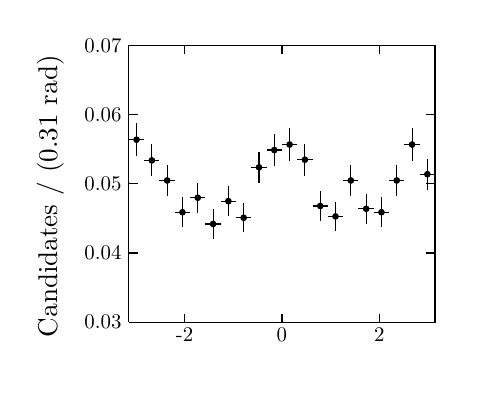
\begin{tikzpicture}
\pgfdeclareplotmark{cross} {
\pgfpathmoveto{\pgfpoint{-0.3\pgfplotmarksize}{\pgfplotmarksize}}
\pgfpathlineto{\pgfpoint{+0.3\pgfplotmarksize}{\pgfplotmarksize}}
\pgfpathlineto{\pgfpoint{+0.3\pgfplotmarksize}{0.3\pgfplotmarksize}}
\pgfpathlineto{\pgfpoint{+1\pgfplotmarksize}{0.3\pgfplotmarksize}}
\pgfpathlineto{\pgfpoint{+1\pgfplotmarksize}{-0.3\pgfplotmarksize}}
\pgfpathlineto{\pgfpoint{+0.3\pgfplotmarksize}{-0.3\pgfplotmarksize}}
\pgfpathlineto{\pgfpoint{+0.3\pgfplotmarksize}{-1.\pgfplotmarksize}}
\pgfpathlineto{\pgfpoint{-0.3\pgfplotmarksize}{-1.\pgfplotmarksize}}
\pgfpathlineto{\pgfpoint{-0.3\pgfplotmarksize}{-0.3\pgfplotmarksize}}
\pgfpathlineto{\pgfpoint{-1.\pgfplotmarksize}{-0.3\pgfplotmarksize}}
\pgfpathlineto{\pgfpoint{-1.\pgfplotmarksize}{0.3\pgfplotmarksize}}
\pgfpathlineto{\pgfpoint{-0.3\pgfplotmarksize}{0.3\pgfplotmarksize}}
\pgfpathclose
\pgfusepathqstroke
}
\pgfdeclareplotmark{cross*} {
\pgfpathmoveto{\pgfpoint{-0.3\pgfplotmarksize}{\pgfplotmarksize}}
\pgfpathlineto{\pgfpoint{+0.3\pgfplotmarksize}{\pgfplotmarksize}}
\pgfpathlineto{\pgfpoint{+0.3\pgfplotmarksize}{0.3\pgfplotmarksize}}
\pgfpathlineto{\pgfpoint{+1\pgfplotmarksize}{0.3\pgfplotmarksize}}
\pgfpathlineto{\pgfpoint{+1\pgfplotmarksize}{-0.3\pgfplotmarksize}}
\pgfpathlineto{\pgfpoint{+0.3\pgfplotmarksize}{-0.3\pgfplotmarksize}}
\pgfpathlineto{\pgfpoint{+0.3\pgfplotmarksize}{-1.\pgfplotmarksize}}
\pgfpathlineto{\pgfpoint{-0.3\pgfplotmarksize}{-1.\pgfplotmarksize}}
\pgfpathlineto{\pgfpoint{-0.3\pgfplotmarksize}{-0.3\pgfplotmarksize}}
\pgfpathlineto{\pgfpoint{-1.\pgfplotmarksize}{-0.3\pgfplotmarksize}}
\pgfpathlineto{\pgfpoint{-1.\pgfplotmarksize}{0.3\pgfplotmarksize}}
\pgfpathlineto{\pgfpoint{-0.3\pgfplotmarksize}{0.3\pgfplotmarksize}}
\pgfpathclose
\pgfusepathqfillstroke
}
\pgfdeclareplotmark{newstar} {
\pgfpathmoveto{\pgfqpoint{0pt}{\pgfplotmarksize}}
\pgfpathlineto{\pgfqpointpolar{44}{0.5\pgfplotmarksize}}
\pgfpathlineto{\pgfqpointpolar{18}{\pgfplotmarksize}}
\pgfpathlineto{\pgfqpointpolar{-20}{0.5\pgfplotmarksize}}
\pgfpathlineto{\pgfqpointpolar{-54}{\pgfplotmarksize}}
\pgfpathlineto{\pgfqpointpolar{-90}{0.5\pgfplotmarksize}}
\pgfpathlineto{\pgfqpointpolar{234}{\pgfplotmarksize}}
\pgfpathlineto{\pgfqpointpolar{198}{0.5\pgfplotmarksize}}
\pgfpathlineto{\pgfqpointpolar{162}{\pgfplotmarksize}}
\pgfpathlineto{\pgfqpointpolar{134}{0.5\pgfplotmarksize}}
\pgfpathclose
\pgfusepathqstroke
}
\pgfdeclareplotmark{newstar*} {
\pgfpathmoveto{\pgfqpoint{0pt}{\pgfplotmarksize}}
\pgfpathlineto{\pgfqpointpolar{44}{0.5\pgfplotmarksize}}
\pgfpathlineto{\pgfqpointpolar{18}{\pgfplotmarksize}}
\pgfpathlineto{\pgfqpointpolar{-20}{0.5\pgfplotmarksize}}
\pgfpathlineto{\pgfqpointpolar{-54}{\pgfplotmarksize}}
\pgfpathlineto{\pgfqpointpolar{-90}{0.5\pgfplotmarksize}}
\pgfpathlineto{\pgfqpointpolar{234}{\pgfplotmarksize}}
\pgfpathlineto{\pgfqpointpolar{198}{0.5\pgfplotmarksize}}
\pgfpathlineto{\pgfqpointpolar{162}{\pgfplotmarksize}}
\pgfpathlineto{\pgfqpointpolar{134}{0.5\pgfplotmarksize}}
\pgfpathclose
\pgfusepathqfillstroke
}
\definecolor{c}{rgb}{1,1,1};
\draw [color=c, fill=c] (5.1,4.72095) rectangle (9.9,9.16419);
\draw [color=c, fill=c] (5.772,5.43186) rectangle (9.66,8.94203);
\definecolor{c}{rgb}{0,0,0};
\draw [c] (5.772,5.43186) -- (5.772,8.94203) -- (9.66,8.94203) -- (9.66,5.43186) -- (5.772,5.43186);
\draw [c,line width=0.4] (5.8692,7.54017) -- (5.8692,7.74857);
\draw [c,line width=0.4] (5.8692,7.74857) -- (5.8692,7.95698);
\draw [c,line width=0.4] (5.772,7.74857) -- (5.8692,7.74857);
\draw [c,line width=0.4] (5.8692,7.74857) -- (5.9664,7.74857);
\foreach \P in {(5.8692,7.74857)}{\draw[mark options={color=c,fill=c},mark size=1.201201pt,mark=*,mark size=1pt] plot coordinates {\P};}
\draw [c,line width=0.4] (6.0636,7.28252) -- (6.0636,7.48531);
\draw [c,line width=0.4] (6.0636,7.48531) -- (6.0636,7.6881);
\draw [c,line width=0.4] (5.9664,7.48531) -- (6.0636,7.48531);
\draw [c,line width=0.4] (6.0636,7.48531) -- (6.1608,7.48531);
\foreach \P in {(6.0636,7.48531)}{\draw[mark options={color=c,fill=c},mark size=1.201201pt,mark=*,mark size=1pt] plot coordinates {\P};}
\draw [c,line width=0.4] (6.258,7.03362) -- (6.258,7.23082);
\draw [c,line width=0.4] (6.258,7.23082) -- (6.258,7.42803);
\draw [c,line width=0.4] (6.1608,7.23082) -- (6.258,7.23082);
\draw [c,line width=0.4] (6.258,7.23082) -- (6.3552,7.23082);
\foreach \P in {(6.258,7.23082)}{\draw[mark options={color=c,fill=c},mark size=1.201201pt,mark=*,mark size=1pt] plot coordinates {\P};}
\draw [c,line width=0.4] (6.4524,6.63915) -- (6.4524,6.82715);
\draw [c,line width=0.4] (6.4524,6.82715) -- (6.4524,7.01516);
\draw [c,line width=0.4] (6.3552,6.82715) -- (6.4524,6.82715);
\draw [c,line width=0.4] (6.4524,6.82715) -- (6.5496,6.82715);
\foreach \P in {(6.4524,6.82715)}{\draw[mark options={color=c,fill=c},mark size=1.201201pt,mark=*,mark size=1pt] plot coordinates {\P};}
\draw [c,line width=0.4] (6.6468,6.81918) -- (6.6468,7.01144);
\draw [c,line width=0.4] (6.6468,7.01144) -- (6.6468,7.2037);
\draw [c,line width=0.4] (6.5496,7.01144) -- (6.6468,7.01144);
\draw [c,line width=0.4] (6.6468,7.01144) -- (6.744,7.01144);
\foreach \P in {(6.6468,7.01144)}{\draw[mark options={color=c,fill=c},mark size=1.201201pt,mark=*,mark size=1pt] plot coordinates {\P};}
\draw [c,line width=0.4] (6.8412,6.49348) -- (6.8412,6.67797);
\draw [c,line width=0.4] (6.8412,6.67797) -- (6.8412,6.86246);
\draw [c,line width=0.4] (6.744,6.67797) -- (6.8412,6.67797);
\draw [c,line width=0.4] (6.8412,6.67797) -- (6.9384,6.67797);
\foreach \P in {(6.8412,6.67797)}{\draw[mark options={color=c,fill=c},mark size=1.201201pt,mark=*,mark size=1pt] plot coordinates {\P};}
\draw [c,line width=0.4] (7.0356,6.77631) -- (7.0356,6.96756);
\draw [c,line width=0.4] (7.0356,6.96756) -- (7.0356,7.15882);
\draw [c,line width=0.4] (6.9384,6.96756) -- (7.0356,6.96756);
\draw [c,line width=0.4] (7.0356,6.96756) -- (7.1328,6.96756);
\foreach \P in {(7.0356,6.96756)}{\draw[mark options={color=c,fill=c},mark size=1.201201pt,mark=*,mark size=1pt] plot coordinates {\P};}
\draw [c,line width=0.4] (7.23,6.57059) -- (7.23,6.75695);
\draw [c,line width=0.4] (7.23,6.75695) -- (7.23,6.94331);
\draw [c,line width=0.4] (7.1328,6.75695) -- (7.23,6.75695);
\draw [c,line width=0.4] (7.23,6.75695) -- (7.3272,6.75695);
\foreach \P in {(7.23,6.75695)}{\draw[mark options={color=c,fill=c},mark size=1.201201pt,mark=*,mark size=1pt] plot coordinates {\P};}
\draw [c,line width=0.4] (7.4244,7.19668) -- (7.4244,7.39756);
\draw [c,line width=0.4] (7.4244,7.39756) -- (7.4244,7.59843);
\draw [c,line width=0.4] (7.3272,7.39756) -- (7.4244,7.39756);
\draw [c,line width=0.4] (7.4244,7.39756) -- (7.5216,7.39756);
\foreach \P in {(7.4244,7.39756)}{\draw[mark options={color=c,fill=c},mark size=1.201201pt,mark=*,mark size=1pt] plot coordinates {\P};}
\draw [c,line width=0.4] (7.6188,7.41133) -- (7.6188,7.61694);
\draw [c,line width=0.4] (7.6188,7.61694) -- (7.6188,7.82256);
\draw [c,line width=0.4] (7.5216,7.61694) -- (7.6188,7.61694);
\draw [c,line width=0.4] (7.6188,7.61694) -- (7.716,7.61694);
\foreach \P in {(7.6188,7.61694)}{\draw[mark options={color=c,fill=c},mark size=1.201201pt,mark=*,mark size=1pt] plot coordinates {\P};}
\draw [c,line width=0.4] (7.8132,7.48004) -- (7.8132,7.68714);
\draw [c,line width=0.4] (7.8132,7.68714) -- (7.8132,7.89425);
\draw [c,line width=0.4] (7.716,7.68714) -- (7.8132,7.68714);
\draw [c,line width=0.4] (7.8132,7.68714) -- (7.9104,7.68714);
\foreach \P in {(7.8132,7.68714)}{\draw[mark options={color=c,fill=c},mark size=1.201201pt,mark=*,mark size=1pt] plot coordinates {\P};}
\draw [c,line width=0.4] (8.0076,7.29111) -- (8.0076,7.49409);
\draw [c,line width=0.4] (8.0076,7.49409) -- (8.0076,7.69706);
\draw [c,line width=0.4] (7.9104,7.49409) -- (8.0076,7.49409);
\draw [c,line width=0.4] (8.0076,7.49409) -- (8.1048,7.49409);
\foreach \P in {(8.0076,7.49409)}{\draw[mark options={color=c,fill=c},mark size=1.201201pt,mark=*,mark size=1pt] plot coordinates {\P};}
\draw [c,line width=0.4] (8.202,6.71629) -- (8.202,6.90613);
\draw [c,line width=0.4] (8.202,6.90613) -- (8.202,7.09597);
\draw [c,line width=0.4] (8.1048,6.90613) -- (8.202,6.90613);
\draw [c,line width=0.4] (8.202,6.90613) -- (8.2992,6.90613);
\foreach \P in {(8.202,6.90613)}{\draw[mark options={color=c,fill=c},mark size=1.201201pt,mark=*,mark size=1pt] plot coordinates {\P};}
\draw [c,line width=0.4] (8.3964,6.58773) -- (8.3964,6.7745);
\draw [c,line width=0.4] (8.3964,6.7745) -- (8.3964,6.96128);
\draw [c,line width=0.4] (8.2992,6.7745) -- (8.3964,6.7745);
\draw [c,line width=0.4] (8.3964,6.7745) -- (8.4936,6.7745);
\foreach \P in {(8.3964,6.7745)}{\draw[mark options={color=c,fill=c},mark size=1.201201pt,mark=*,mark size=1pt] plot coordinates {\P};}
\draw [c,line width=0.4] (8.5908,7.03362) -- (8.5908,7.23082);
\draw [c,line width=0.4] (8.5908,7.23082) -- (8.5908,7.42803);
\draw [c,line width=0.4] (8.4936,7.23082) -- (8.5908,7.23082);
\draw [c,line width=0.4] (8.5908,7.23082) -- (8.688,7.23082);
\foreach \P in {(8.5908,7.23082)}{\draw[mark options={color=c,fill=c},mark size=1.201201pt,mark=*,mark size=1pt] plot coordinates {\P};}
\draw [c,line width=0.4] (8.7852,6.682) -- (8.7852,6.87103);
\draw [c,line width=0.4] (8.7852,6.87103) -- (8.7852,7.06006);
\draw [c,line width=0.4] (8.688,6.87103) -- (8.7852,6.87103);
\draw [c,line width=0.4] (8.7852,6.87103) -- (8.8824,6.87103);
\foreach \P in {(8.7852,6.87103)}{\draw[mark options={color=c,fill=c},mark size=1.201201pt,mark=*,mark size=1pt] plot coordinates {\P};}
\draw [c,line width=0.4] (8.9796,6.63915) -- (8.9796,6.82715);
\draw [c,line width=0.4] (8.9796,6.82715) -- (8.9796,7.01516);
\draw [c,line width=0.4] (8.8824,6.82715) -- (8.9796,6.82715);
\draw [c,line width=0.4] (8.9796,6.82715) -- (9.0768,6.82715);
\foreach \P in {(8.9796,6.82715)}{\draw[mark options={color=c,fill=c},mark size=1.201201pt,mark=*,mark size=1pt] plot coordinates {\P};}
\draw [c,line width=0.4] (9.174,7.03362) -- (9.174,7.23082);
\draw [c,line width=0.4] (9.174,7.23082) -- (9.174,7.42803);
\draw [c,line width=0.4] (9.0768,7.23082) -- (9.174,7.23082);
\draw [c,line width=0.4] (9.174,7.23082) -- (9.2712,7.23082);
\foreach \P in {(9.174,7.23082)}{\draw[mark options={color=c,fill=c},mark size=1.201201pt,mark=*,mark size=1pt] plot coordinates {\P};}
\draw [c,line width=0.4] (9.3684,7.48004) -- (9.3684,7.68714);
\draw [c,line width=0.4] (9.3684,7.68714) -- (9.3684,7.89425);
\draw [c,line width=0.4] (9.2712,7.68714) -- (9.3684,7.68714);
\draw [c,line width=0.4] (9.3684,7.68714) -- (9.4656,7.68714);
\foreach \P in {(9.3684,7.68714)}{\draw[mark options={color=c,fill=c},mark size=1.201201pt,mark=*,mark size=1pt] plot coordinates {\P};}
\draw [c,line width=0.4] (9.5628,7.11085) -- (9.5628,7.3098);
\draw [c,line width=0.4] (9.5628,7.3098) -- (9.5628,7.50875);
\draw [c,line width=0.4] (9.4656,7.3098) -- (9.5628,7.3098);
\draw [c,line width=0.4] (9.5628,7.3098) -- (9.66,7.3098);
\foreach \P in {(9.5628,7.3098)}{\draw[mark options={color=c,fill=c},mark size=1.201201pt,mark=*,mark size=1pt] plot coordinates {\P};}
\draw [c,line width=0.4] (5.772,5.43186) -- (9.66,5.43186);
\draw [anchor= east] (9.66,4.93422) node[scale=0.979298, rotate=0]{$\phihel$};
\draw [c,line width=0.4] (6.47841,5.53984) -- (6.47841,5.43186);
\draw [c,line width=0.4] (7.716,5.53984) -- (7.716,5.43186);
\draw [c,line width=0.4] (8.95359,5.53984) -- (8.95359,5.43186);
\draw [c,line width=0.4] (6.47841,5.53984) -- (6.47841,5.43186);
\draw [c,line width=0.4] (8.95359,5.53984) -- (8.95359,5.43186);
\draw [anchor=base] (6.47841,5.19193) node[scale=0.753306, rotate=0]{-2};
\draw [anchor=base] (7.716,5.19193) node[scale=0.753306, rotate=0]{0};
\draw [anchor=base] (8.95359,5.19193) node[scale=0.753306, rotate=0]{2};
\draw [c,line width=0.4] (5.772,8.94203) -- (9.66,8.94203);
\draw [c,line width=0.4] (6.47841,8.83406) -- (6.47841,8.94203);
\draw [c,line width=0.4] (7.716,8.83406) -- (7.716,8.94203);
\draw [c,line width=0.4] (8.95359,8.83406) -- (8.95359,8.94203);
\draw [c,line width=0.4] (6.47841,8.83406) -- (6.47841,8.94203);
\draw [c,line width=0.4] (8.95359,8.83406) -- (8.95359,8.94203);
\draw [c,line width=0.4] (5.772,5.43186) -- (5.772,8.94203);
\draw [anchor= east] (4.7736,8.94203) node[scale=0.979298, rotate=90]{Candidates / (0.31 rad)};
\draw [c,line width=0.4] (5.88576,5.43186) -- (5.772,5.43186);
\draw [c,line width=0.4] (5.88576,6.30941) -- (5.772,6.30941);
\draw [c,line width=0.4] (5.88576,7.18695) -- (5.772,7.18695);
\draw [c,line width=0.4] (5.88576,8.06449) -- (5.772,8.06449);
\draw [c,line width=0.4] (5.88576,8.94203) -- (5.772,8.94203);
\draw [anchor= east] (5.772,5.43186) node[scale=0.753306, rotate=0]{0.03};
\draw [anchor= east] (5.772,6.30941) node[scale=0.753306, rotate=0]{0.04};
\draw [anchor= east] (5.772,7.18695) node[scale=0.753306, rotate=0]{0.05};
\draw [anchor= east] (5.772,8.06449) node[scale=0.753306, rotate=0]{0.06};
\draw [anchor= east] (5.772,8.94203) node[scale=0.753306, rotate=0]{0.07};
\draw [c,line width=0.4] (9.66,5.43186) -- (9.66,8.94203);
\draw [c,line width=0.4] (9.54624,5.43186) -- (9.66,5.43186);
\draw [c,line width=0.4] (9.54624,6.30941) -- (9.66,6.30941);
\draw [c,line width=0.4] (9.54624,7.18695) -- (9.66,7.18695);
\draw [c,line width=0.4] (9.54624,8.06449) -- (9.66,8.06449);
\draw [c,line width=0.4] (9.54624,8.94203) -- (9.66,8.94203);
\end{tikzpicture}
